\thispagestyle{empty}

\section{Theorie}



\subsection{Container}
Container-basierte Virtualisierung ist ein leichtgewichtiger Virtualisierungsansatz auf Betriebssystemebene, bei dem der Host-Kernel zur Ausführung mehrerer virtueller Umgebungen verwendet wird. Diese virtuellen Umgebungen werden oft einfach als \glqq Container \grqq{} bezeichnet. Linux-V Server[X], Open VZ\cite{IndexOpenvz.org} und Linux Container(LXC)\cite{IndexLinuxcontainers.Org} sind die drei wichtigsten Vertreter dieses Ansatzes. Die allgemeine Architektur einer Container-basierten Virtualisierungslösung ist in Abbildung \ref{fig:architecture} dargestellt. Containerbasierte Virtualisierung erfolgt auf Betriebssystem Ebene, so dass mehrere Anwendungen ohne redundante Ausführung anderer Betriebssysteme auf dem Host betrieben werden können. Container sehen von außen aus wie normale Prozesse, die auf dem Kernel laufen, der mit dem Host-Rechner geteilt wird. Sie stellen eine isolierte Umgebung mit den notwendigen Ressourcen für die Ausführung von Anwendungen zur Verfügung. Diese Ressourcen können entweder mit dem Host geteilt oder separat im Container installiert werden \cite{Xavier2014AClusters}. Namespaces sind die Basis des LXC und stellen in Verbindung mit anderen Ressourcen-Management-Systemen eine isolierte Umgebung in Form von Containern zu Verfügung. LXC nimmt die cgroups Ressourcenverwaltungseinrichtungen\cite{Heo2015ControlV2} als Grundlage und fügt POSIX file Capabilities [X] hinzu, um die Ressourcen unter den Containern einzuschränken. 

\vspace{1em}
\begin{minipage}{\linewidth}
	\centering
	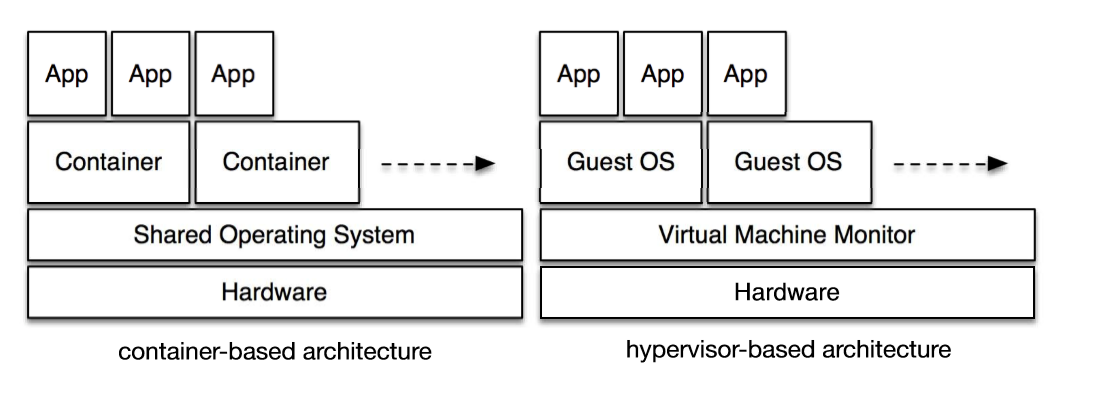
\includegraphics[width=1\linewidth]{pics/docker2.png}
	\captionof{figure}[Architektur]{Aufbau Container und Virtuelle Maschine \cite{Xavier2015AClouds}}
	\label{fig:architecture}
\end{minipage}

\subsubsection{Namespaces drüberschauen buch seite 68}
Seit der Einführung der Kernel Namespaces ist es möglich, Ressourcen des Kernsystems  voneinander zu isolieren und diese Teile unter bestimmten Voraussetzungen anderen Anwendungen/Prozessen zur Verfügung zu stellen. 

Wenn man sich die zugrunde liegenden Funktionsaufrufe anschaut erkennt man, dass fast alle Namespaces via clone- und stnsOperationen zur Verfügung gestellt werden. Für den oder die Prozesse innerhalb eines Namespaces ist dies jedoch nicht erkennbar. Der innerhalb eines Namespaces gestatete Prozessaufruf arbeitet isoliert und sieht nur sich selbst und seine Kindprozesse, jedoch nicht die übergeordnete Umgebung, während der übergeordnete Prozess natürlich alle Namespaces und darin laufende Prozesse sieht. 

Derzeit existieren sechs verschiedene Namensräume, unter anderem der PID Namespace. Dieser kann uns über die Namespace-Abschottung z.B. einen sogenannten nested Process Tree zur Verfügung stellen, also einen gekapselten Prozessbaum innerhalb des eigentlichen (Host-)Prozessbaumes, in welchem unsere Container-Instanz läuft. Aber dies ist nicht der einzige Namspace, an dem unsere Container partizipieren dürfen.

Die vereinfachte Darstellung des PID Namespaces einer gespawnten bzw geforkten Container-Prozess-Umgebung ist in Abbildung \ref{fig:PID} dargestellt. \cite{Liebel2017SkalierbareContainer-Infrastrukturen}

\vspace{1em}
\begin{minipage}{\linewidth}
	\centering
	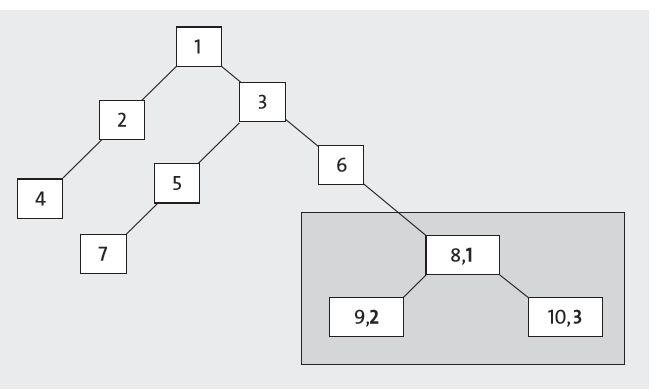
\includegraphics[width=1\linewidth]{pics/PID.PNG}
	\captionof{figure}[PID]{ PID Namespaces für Host und Container (im Fettdruck) \cite{Liebel2017SkalierbareContainer-Infrastrukturen}}
	\label{fig:PID}
\end{minipage}

\subparagraph{PID-Namespace} ist hierarchisch[X] deshalb kann ein Prozess nur die anderen Prozesse in seinem eigenen Namensraum oder in seinen untergeordneten Namensräumen sehen. Folglich kann der Host die Prozesse innerhalb des neuen PID-namespace des Containers beobachten und beeinflussen, aber die Prozesse innerhalb des Containers können die anderen Prozesse, die im Host oder in anderen Containern laufen, nicht beobachten oder beeinflussen

\subparagraph{Mount-Namespace} isoliert filesystem Mountpunkte, die von einem Container gesehen werden, so dass Prozesse in verschiedenen Containern unterschiedliche Ansichten der file Systemhierarchie haben können.

\subparagraph{UTS-Namespace} erlaubt es jedem Container seinen eigenen Hostnamen und NIS-Domänennamen zu haben.

\subparagraph{IPC-Namespace} isoliert die Interprozesskommunikation, das bedeutet Prozesse, die in einem Container enthalten sind, haben eigene Nachrichten Warteschlangen und sind völlig unabhängig von Prozessen in anderen Containern.

\subparagraph{Network namespace} isoliert das Netzwerk-Untersystem wie z.B. Geräte und IP-Adressen. Jeder Container unterhält seine eigene Netzwerk Konfiguration und die darauf laufenden Anwendung.

\subparagraph{User-Namespace} isoliert Benutzer-IDs vom Host und anderen laufenden Containern. Das bedeutet, dass der Benutzer root (ID0) innerhalb eines Containers volle Privilegien hat, aber keine Privilegien außerhalb, was Sicherheit und Zuverlässigkeit gewährleistet. \cite{Xavier2015AClouds}
	



\subsubsection{cgroup}
\glqq c-group\grqq{} steht für \glqq contol group\grqq{}. Durch cgroup ist es möglich, eine Reihe von Kriterien anzuwenden, um Ressourcen wie Speicher,Netzwerk, Festplatten-I/O und CPU einzuschränken. Ein Container sollte seine auferlegten Beschränkungen nicht überschreiten und andere Container, die auf derselben Hardware laufen, nicht stören. Cgroup ist für die Ressourcen Begrenzung, Priorisierung, Abrechnung und Kontrolle zuständig.\cite{Heo2015ControlV2} 

cgroup ist ein Mechanismus, um Prozesse und System Ressourcen entlang der Hierarchie in einer kontrollierten und konfigurierbaren weise hierarchisch zu organisieren. cgroup besteht im Wesentlichen aus zwei Teilen, dem Kern und dem Controller. Der cgroup Kern ist in erster Linie für die hierarchische Organisation von Prozessen zuständig. Der cgroup Controller ist in der Regel für die Verteilung einer bestimmten Art von System Ressource entlang der Hierarchie verantwortlich. Cgroup bilden eine Baumstruktur und jeder Prozess im System gehört genau zu einer cgroup. Alle Unterprozesse (Kind Prozesse) eines Prozesses (Eltern Prozess) gehören zur gleichen cgroup. Alle neu erstellten Prozesse gehören zu der cgroup zu der auch der Eltern Prozess gehört.


\paragraph{Ressourcen Verteilungs Modelle}
Cgroup Controller verfügen über verschiedene Ressourcen Verteilungs Modelle. Die Modelle sind auf die Art und den Verwendungszweck der Ressource zugeschnitten. Dieser Paragraph befasst sich mit den verschiedenen Hauptschemen und deren Aufgaben.

----CPU kann kein Prozent wert zugeteilt werden weil durch eine geringe Auslastung die Leistung runter fährt (youtube video siehe one noteJérôme Petazzoni )

\subparagraph{Weight}
Die Ressourcen eines Prozesses werden Proportional an alle aktiven Kind Prozesse verteilt. Da nur die aktiven Kind Prozesse welche aktuell Ressourcen benötigen an der Verteilung teilnehmen, werden die zugeteilten Ressourcen effizient genutzt. 

Alle Konfigurationen sind gültig und es gibt keinen Grund, Migrationen von Konfigurationsänderungsprozessen abzulehnen.

\subparagraph{Limit}
Ist ein High-Limit gesetzt, kann ein Kind Prozess nur bis zu der konfigurierten Menge einer Ressource Verwenden. Low/High Limits können auch als soft-Limits bezeichnet werden. Die Summe der Limits aller Kind Prozesse kann die zur Verfügung stehende Menge an Ressourcen des Eltern Prozesses überschreiten. Ein Limit ist sozusagen ein maximaler Richtwert der bei dringendem Bedarf überschritten werden kann. Der Prozess welcher den über das Limit hinaus ragende Anteil verwendet, steht unter erhöhtem Druck und wird gedrängt die Ressource schnell wieder frei zu geben. Wenn eine cgroup die Ressourcen nicht mehr benötigt, wird diese bis zu einem setzbaren Low-Limit freigegeben.

Da Limits überschritten werden können, sind alle Konfigurationen gültig und es gibt keinen Grund Konfigurationsänderungen zurück zu weisen.

\subparagraph{Protection}
Eine cgroup ist so geschützt, dass sie bis zur konfigurierten Menge der Ressource fest zugeordnet werden kann, wenn die Verwendung aller Prozesse unter der geschützten Ebene Liegt. Der Schutz kann garantiert oder effizient sein. Bei garantiertem Schutz wird die Ressource explizit für die cgroup frei gehalten und kann vollständig verwendet werden. Die Effizientere Variante bietet die Möglichkeit zugeteilte Ressourcen auf Anfrage für andere Prozesse frei zu stellen.

Die Protectionen können überschritten werden somit sind alle Konfigurationsmethoden gültig.

\subparagraph{Allocation}
Einer cgroup wird eine bestimmte Menge einer Ressource fest zugeteilt und stellt somit ein Hard-Limit dar. Die Summe der Zuweisungen von Kind Prozessen dürfen die Menge der fest zugeteilten Ressource des Eltern Prozesses nicht überschreiten. Auch wenn die Ressource nicht ausgenutzt wird, bleibt diese der cgroup erhalten. 

Es gibt bei Allocationen einige Konfigurationen die zurückgewiesen werden. Wenn bei der Bildung eines neuen Prozesses die zur Ausführung benötige Ressourcenmenge überschritten werden, wird der Prozess verworfen.

\paragraph{Ressourcen Modellierung}
Im folgenden Paragraphen werden Art der Ressource mit verwendetem Modell aufgelistet

\subparagraph{Speicher}
Der Speicher Controller regelt die Verteilung des Speichers. Speicher ist zustandsabhängig und verwendet sowohl Limit als auch Protection Modelle. Aufgrund der Verflechtung zwischen Speicherbedarf und Speicherrückgabeforderung ist die Verwaltung sehr kompliziert.

Memory-low(Best-effort)
Der geforderte Mindestanteil wird gestellt. Unbenutzer Speicher kann bei Bedarf vom System verwendet werden.

Memory-High(Best-effort)
Dies ist der Hauptmechanismus zur Steuerung des Speicherverbrauchs einer cgroup. WEnn die Nutzung einer cgroup über die obere Grenze hinausgeht, werden die Prozesse der cgroup gedrosselt und unter starken Reklamationsdruck gesetzt.

Memory-min(Hard-Limit)
Falls der Speicherverbrauch einer cgroup innerhalb seiner effektiven minimalen Grenze liegt, wird der Speicher der cgroup unter keinen Umständen zurückgefordert. Wenn nicht genug Speicherplatz zur Verfügung steht um die Minimalanforderung zu gewährleisten, kommt der OOM-Killer zum Einsatz und schafft freien Speicher.

Memory-max(Hard-Limit)
Wenn der Speicherverbrauch einer cgroup diese Grenze erreicht und nicht reduziert werden kann, wird der OOM-Killer in der cgroup aufgerufen, dies ist der letzte Schutzmechanismus. Unter bestimmten Umständen kann ein Prozess vorübergehend über das Limit hinaus gehen.

\subparagraph{CPU}
Der CPU Controller reguliert die Verteilung der CPU-Zyklen. Diese Steuerung Verwendet Gewichtung und Limit Modelle für normale Ressourcen Verteilung und das Allocation Modell für eine Echtzeit Verteilung.

Die CPU kann nicht auf einen genauen gleichbleibenden Prozentwert angegeben werden, da sich die Leistung der CPU aus Energie Effizienz gründen an die Auslastung anpasst.

\subparagraph{IO}
Der IO Controller reguliert die Verteilung der IO Ressourcen. Der Controller verwendet Gewichtung und Limit Modelle. Die Gewichtung gibt die relative IO-Zeit and, die die cgroup in Bezug auf ihre Geschwister verwenden kann.


\subsection{Virtuelle Maschine}
Eine Virtuelle Maschine Bildet mit Hilfe des Virtuellen Maschinen Monitors (VMM)/Hypervisor eine komplette Rechnerarchitektur auf dem Host-Rechner nach (siehe Abbildung \ref{fig:architecture}). Man unterscheidet zwischen zwei Arten von VMM: Dem Typ 1 VMM oder "Bare-Metal-Hypervisor" genannt, welcher direkt auf der zugrundeliegenden Hardware des Hosts liegt und dem Typ-2-VMM "gehosteter Hypervisor" welcher eine komplette virtuelle Maschine auf dem Host Betriebssystem erstellt. Die Grundanforderung eines VMM sind nach Popek/Goldberg (1974) \cite{Popek1974FormalArchitectures,Glatz2015Betriebssysteme} :

\subparagraph{Ausführungsumgebung}
Prozesse welche auf der Virtuellen Maschine gestartet wurden, laufen mit Ausnahme der Geschwindigkeit identisch ab, wie Prozesse auf einem originalen Host-System.

\subparagraph{Effizienz}
Die meisten Prozesse werden von der Hardware direkt ausgeführt ohne eingreifen des VMM

\subparagraph{Ressourcenverwaltung}

Es darf kein Prozess Ressourcen verwalten. Bei jedem zugriffsversuch eines Prozesses auf Systemressourcen wird der VMM aufgerufen.

\subsubsection{Typ-1-VMM}
Der VMM Liegt direkt auf der Hardware mit vollen Zugriffsrechten, kümmert sich um die Ressourcenverwaltung und die Isolierte Bereitstellung von Virtuellen Maschinen und stellt ein eigenes Betriebssystem dar (siehe Abbildung \ref{fig:Hypervisor_Typ1/Typ2} a) . Die Aufteilung der Rechenzeit und die Zuteilung von Speicher auf die einzelnen VMs sind beispiele der Aufgaben welche die Ressourcenverwaltung übernimmt. VMware ESX [X] ist ein Beispiel für diesen Virtuallisierungs Ansatz, das mit einem eigenen Treiber nur direkt auf der Hardware laufen kann.

\vspace{1em}
\begin{minipage}{\linewidth}
	\centering
	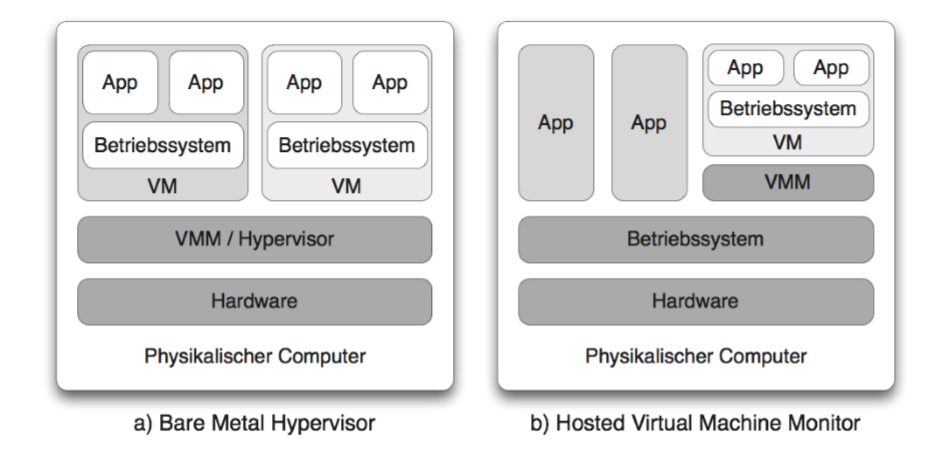
\includegraphics[width=1\linewidth]{pics/Hypervisoren.PNG}
	\captionof{figure}[Hypervisor Typ1/Type2]{Hypervisor Typ1/Typ2 \cite{Meinel2011VirtualisierungMarktubersicht} }
	\label{fig:Hypervisor_Typ1/Typ2}
\end{minipage}

\subsubsection{Typ-2-VMM}
Ein Typ-2-VMM teilt sich ein Gastgeberbetriebssystem(Host) mit anderen Applikationen (siehe Abbildung \ref{fig:Hypervisor_Typ1/Typ2} b). Um die nötigen Rechte auf der Hardware zu erhalten, wird ein spezieller VMM-Treiber verwendet, der direkt unter dem Host-system installiert wird. Dieser ermöglicht Privilegierte Zugriffsrechte auf den Kernel \cite{Glatz2015Betriebssysteme}.


\subsubsection{Rechteverwaltung}
Egal, welche Methode der Virtualisierung zum Einstz kommt, eins haben sie gemeinsam: Einige Befehle, die das Gastsystem an die CPU sendet, müssen von der Virtualisierungsschicht abgefangen und interpretiert werden \cite{Glatz2015Betriebssysteme}. Das geschieht entweder über \glqq binary translation \grqq{} oder Via Hypercalls. 

 Es gibt bei aktuellen Prozessoren eine Rechteverwaltung welche man als Ringdiagramm darstellen kann (siehe Abbildung \ref{fig:Ringmodell1} b).Im Ring 0 Besitzt man Volle Zugriffsrechte auf Hardware Ressourcen, auf dieser Ebene ist der Kernel beheimatet. Die Ringe 1 und 2 stehen für Treiber zur Verfügung und im Ring 3 Stehen alle sonstigen Anwendungen. Die Kernel der Gastbetriebssysteme befinden sich ebenfalls in dem 3. Ring. Wenn eine Anwendung direkt auf einen Speicherbereich zugreifen will, der vom Kernel reserviert ist, tritt eine Speicherschutzverletzung auf und der Zugriff wird verweigert, was den Prozess abstürzen lässt. Der Hypervisor fängt solche kritischen Anfragen ab überprüft diese, Codiert die Anfragenstellung gegebenenfalls um und führt sie selbst aus. Nach dem Aufruf folgt eine entsprechende Rückübersetzung und Rückabe an die aufrufende virtuelle Maschine. Dieser Vorgang heist \glqq binary translation \grqq{} und muss sehr häufig durchgeführt werden, was zu einem Overhead, der erhöhte Leistungseinbußen zur Folge hat. 
 
 
 \vspace{1em}
\begin{minipage}{\linewidth}
	\centering
	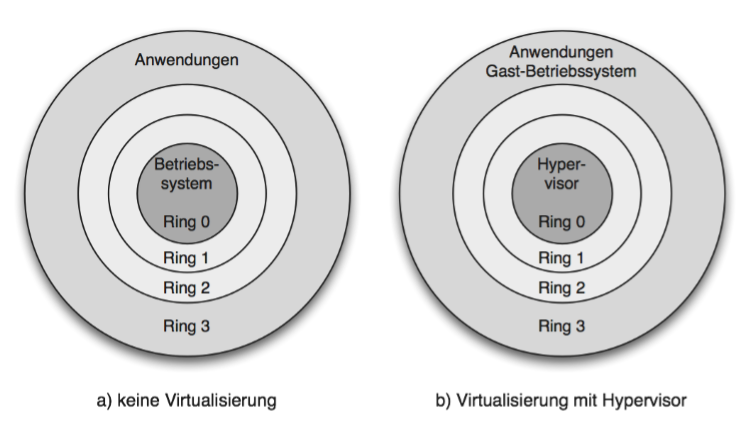
\includegraphics[width=1\linewidth]{pics/Ringmodell1.PNG}
	\captionof{figure}[Ringmodell 1 ]{Rechteverwaltung \cite{Meinel2011VirtualisierungMarktubersicht} }
	\label{fig:Ringmodell1}
\end{minipage}
 
 
 
 Für Hypercalls benötigt man eine Paravirtuallisierung die zwischen Typ 1 VMM und Typ2 VMM einzuordnen ist. Hierzu muss muss ein Hypervisor von Haus aus bereits in das Betriebssystem integriert sein, außerdem werden die Kernel der Gastbetriebssysteme so angepasst, dass diese auf Ring 1 laufen können (siehe Abbildung \ref{fig:Ringmodell2}). Aus Systemaufrufen werden nun Hypercalls direkt an den Hypervisor und nicht wie vorher an die Hardware. Der Hypervisor führt den entsprechenden Systemaufruf aus und bedient die aufrufende virtuelle Maschine \cite{Glatz2015Betriebssysteme} \cite{Meinel2011VirtualisierungMarktubersicht}. KVM(Kernel-based Virtual Mashine) ist der Vertreter dieses Ansatzes auf Linux Seite und durch Hyper-V wird dieser auf Windows Realisiert. 



 \vspace{1em}
\begin{minipage}{\linewidth}
	\centering
	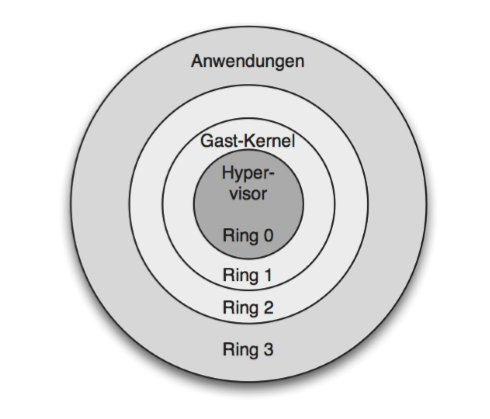
\includegraphics[width=0.5\linewidth]{pics/Ringmodell2.PNG}
	\captionof{figure}[Ringmodell 2 ]{Rechteverwaltung Paravirtuallisierung \cite{Meinel2011VirtualisierungMarktubersicht} }
	\label{fig:Ringmodell2}
\end{minipage}
 





Virtuallisierungen
Vollstendige virtuallisierung 
Paravirtualisierung

Hyper-V
KVM

Kernel
OOM Killer

%\pagebreak